\chapter{Literature Review}
\label{sec:Literature Review}

 This section of the report documents the relevant research performed.

\section{Laparoscopy Overview}
\label{sec:Laparoscopy Overview}

Laparoscopy is a branch of endoscopy. It has become an integral part of surgical procedures in all surgical fields in recent decades. Inspired by the minimally invasive surgery (MIS) approach, laparoscopic surgery consists of making one or more small incisions in the abdomen of the patient. Surgeons use these incisions to insert thin, rod-like medical equipment into the patient to perform the surgery. \citep{FIS-2021}

An essential tool of this surgical procedure is the laparoscope. Due to the small incisions, the surgeon's view is limited. The laparoscope is the solution to this problem. It allows surgeons to view the interior within the patient as the operation is being performed. Therefore, they can clearly manipulate their equipment from outside the patient to perform complex procedures inside the patient. \citep{AIP-2018}

Modern laparoscopes are equipped with small cameras and light sources at the end of the tool. This camera is inserted into the patient, and the captured footage is displayed immediately to the surgical staff on a monitor. With the visible footage, the surgical staff can make a diagnosis and perform operations. \citep{AIP-2018}

However, the first laparoscope was invented a century ago. They did not consist of cameras, but rather, of complex lens assemblies at the end of the laparoscope and cold light sources. They were used in a similar method to a microscope. However, this severely limited the surgeon’s ability to operate and the surgical staff’s ability to assist the operating surgeon. \citep{FIS-2021} Figure \ref{fig:old laparoscope} illustrates how the original laparoscope was designed.

\begin{figure}[H]
    \centering
    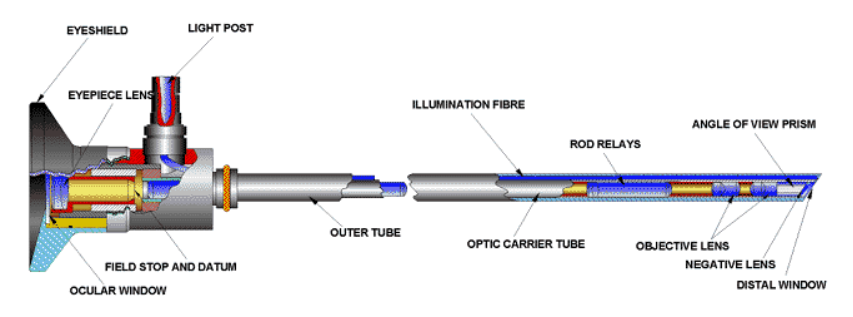
\includegraphics[height = 5cm]{figs/Endoscope.png}
    \caption{Original laparoscope design. \citep{EBME-2026}}
    \label{fig:old laparoscope}
\end{figure}


Laparoscopic surgery has been one of the greatest advancements in the medical industry in recent years.  \citet{WJM-2015} show that laparoscopic surgery has a quicker recovery time and less pain after surgery compared to traditional open surgery. However, it shows that certain procedures are more time‑consuming and complex to perform. 


\section{Current Available Technology}
\label{sec:Current Available Technology}

There is a range of laparoscopes or endoscopes suppliers across the globe. Each of these suppliers produces more than one product. Therefore, only local suppliers will be reviewed, as well as Intuitive Surgical, which produces the Da Vinci system, which has dominated the surgical robot market. \citep{AIP-2018}

One of the main suppliers of laparoscopic equipment in South Africa is Karl Storz Endoskope, a German company, with a sales office in Cape Town. They produce numerous products in the medical industry. \citep{KSE-HP} One of their products is the \textit{TIPCAM1 RUBINA}, illustrated in Figure \ref{fig:TIPCAM1}.

\textit{TIPCAM1 RUBINA} is a rigid endoscope with a viewing angle of either 0° or 30°. It comes with automatic horizon control and the ability to easily swap between 2D and 3D imaging. It has an outer diameter of 10.3~mm and a working length of 320~mm. Additionally, it has a 4K image resolution and a mass of 420~g. \citep{KSE-TR}


\begin{figure}[H]
    \centering
    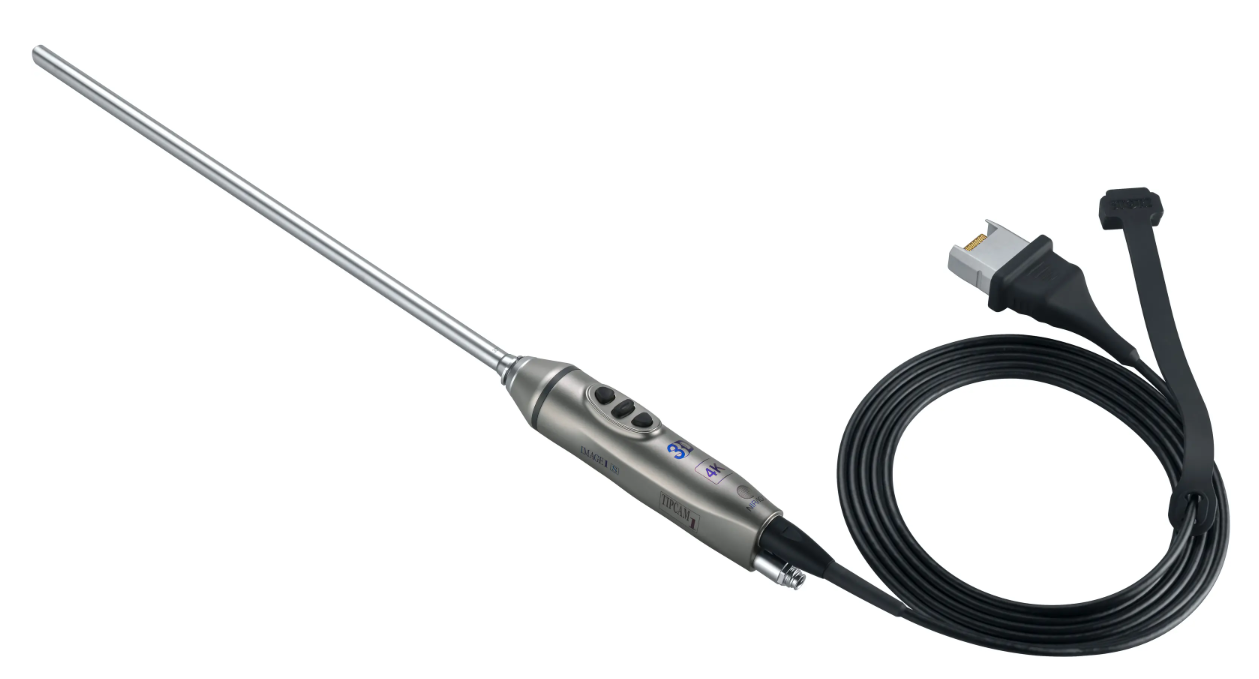
\includegraphics[width=0.5\linewidth]{figs/TIPCAM1 RUBINA.png}
    \caption{Figure of the TIPCAM1 RUBINA. \citep{KSE-TR}}
    \label{fig:TIPCAM1}
\end{figure}

Olympus Corporation is another company that supplies medical equipment globally. They are a Japanese manufacturing company that produces the \textit{ENDOEYE 3D 10 mm}, which can be seen in Figure \ref{fig:ENDOEYE}. The \textit{ENDOEYE 3D 10 mm} is a video telescope, with the ability of 3D imaging at a viewing angle of 0° and 30°. It is able to perform image rotation at 30° viewing angle while maintaining the horizon. \citep{OC-E}

\begin{figure}[htpb]
    \centering
    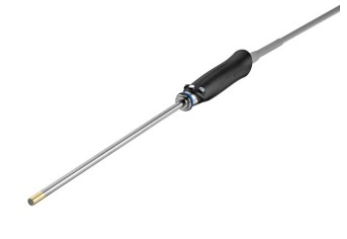
\includegraphics[width=0.5\linewidth]{figs/ENDOEYE 3D 10mm.png}
    \caption{Figure of the ENDOEYE 3D 10 mm. \citep{OC-E}}
    \label{fig:ENDOEYE}
\end{figure}

Certain international companies use local distributors to sell their products. Intuitive Surgery, an American company, uses this method. They designed and manufactured the \textit{Da Vinci} medical robot. This system has various variants for different surgical purposes. Currently, there are \textit{Da Vinci Xi} and \textit{Da Vinci X} for multi-port surgery. However, the \textit{Da Vinci SP} is designed for single-port surgery. These robot systems are equipped with seven DOF movement and 3D visualization. Their main drawback is their large size and enormous financial procurement and maintenance cost. \citep{IS-SP} Below in Figure \ref{fig:Da Vinci} the \textit{Da Vinci SP} is illustrated.

\begin{figure}[H]
    \centering
    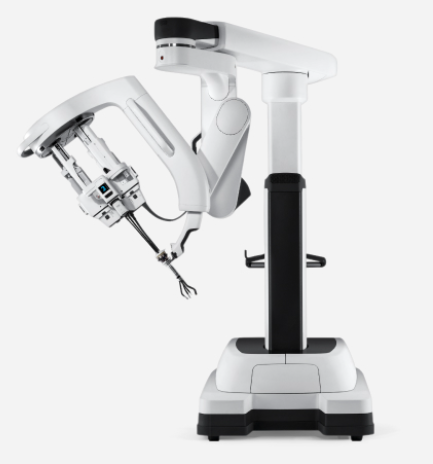
\includegraphics[width=0.5\linewidth]{figs/Da Vinci SP.png}
    \caption{Figure of the Da Vinci SP. \citep{IS-SP}}
    \label{fig:Da Vinci}
\end{figure}

\section{Current Technological Advancements}
\label{sec:Current Technological Advancements}

Since the addition of cameras to laparoscopes, there have been significant opportunities for advancements. These advancements range from hardware improvements to software additions to the existing design. 

 The main hardware advancement for laparoscopes is the improvement of camera modules. However, more advancements have been made with the addition of robotics to the laparoscopes, which have greatly assisted the laparoscopic surgical industry. Robotic manipulators are utilized to assist surgeons by maintaining stable control of the laparoscope. Therefore, ensuring consistent and clear visualization during the procedure. \citep{AIP-2018}

 There are multiple additions currently being made to the software application of laparoscopes. \citet{AIP-2018} list the following additions: 

\begin{itemize}
    \item Digital imaging enhancement techniques.
    \item AI incorporation.
    \item 3D visualization.
    \item Object tracking.
\end{itemize}

\section{Available Hardware Components}
\label{sec:Available Hardware Components}

This section will be divided into multiple subsections where different products will be reviewed for each component. These subsections are:

\begin{itemize}
    \item \hyperref[sec:Main Microcontroller and Computer Module]{Single board computer module.}
    \item \hyperref[sec:Camera Module]{Camera module.}
    \item \hyperref[sec:Lighting Module]{Lighting module.}
    \item \hyperref[sec:Heat Components]{Heat transfer components}
\end{itemize}

\subsection{Single Board Computer Module}
\label{sec:Main Microcontroller and Computer Module}

 Single-board computers (SBCs) are credit‑card‑size computers, able to perform complex computations while operating various systems. For the laparoscope, it will be the main "brain" of the system. Therefore, it is critical that it can perform all the necessary tasks it requires. There are two main suppliers of SBC: 


\begin{itemize}
    \item Raspberry Pi Ltd.
    \item Arduino AG.
\end{itemize}

Raspberry Pi has a large range of products that are available for the project. However, Raspberry Pi’s SBCs have an important feature, which would be beneficial to the project. This feature is the designated camera serial interface (CSI) or the MIPI camera display transceivers, according to Raspberry Pi. This feature allows for high‑quality videos at high frame rates. \citep{RP-DOC} Table \ref{tab:Raspberry Pi SBC} shows the available options of all the Raspberry Pi SBCs:

\begin{table}[H]
    \centering
    \caption{Raspberry Pi SBCs. \citep{RP-P}}
    \begin{tabular}{|c|c|c|c|c|}
    \hline
        Raspberry Pi SBC & RAM & CPU Speed & MIPI Ports & Cost \\
    \hline
        Pi 5 & 1-16 GB & 2.4 GHz & 2 & R 3 266.00\\
    \hline
        Pi 4 Model B & 1-8 GB & 1.5 GHz & 1 & R 1 360.00\\
    \hline
        Pi 3 Model B+ & 1 GB & 1.4 GHz & 1 & R 640.43\\
    \hline
        Pi Zero 2 W & 512 MB & 1 GHz & 2 & R 240.16 \\ 
    \hline
        Pi Zero 2 & 512 MB & 1 GHz & 2 & R 309.90 \\ 
    \hline
    \end{tabular}
    \label{tab:Raspberry Pi SBC}
\end{table}

All the SBCs listed in Table \ref{tab:Raspberry Pi SBC} have these features:

\begin{itemize}
    \item 40 General-Purpose Input/Output (GPIO) pins.
    \item Wi-Fi capabilities.
    \item Bluetooth capabilities.
    \item USB ports.
\end{itemize}

Arduino, similar to Raspberry Pi, has a wide range of products available for this project. However, they lack a CSI port. Therefore, they are incompatible with the Raspberry Pi camera modules. Additionally, they also have much lower RAM than the Raspberry Pi SBC's. Therefore, they were not considered for this project.  \citep{GH-AA}

%However, they can use other camera modules, with the use of SPI and I2C GPIO pins. Although this option isn’t favourable, due to a trade‑off in quality during longer videos, it is still a feasible option that can be explored. \citep{GH-AA} The Table \ref{tab:Arduino SBCs} below shows the available products from Arduino:

% \begin{table}[H]
%     \centering
%     \caption{Arduino SBCs. \citep{A-P}}
%     \begin{tabular}{|c|c|c|c|c|}
%         \hline
%             Arduino SBC & RAM & CPU Speed & SPI Ports & Cost \\
%         \hline
%             UNO R4 WiFi & 32 kB & 48 MHz & 1 & R 488.46 \\
%         \hline 
%             UNO R4 Minima & 32 kB & 48 MHz & 1 & R 352.33 \\
%         \hline
%             UNO R3 & 2 kB & 16 MHz & 1 & R 469.24\\
%  %       \hline
% %            Mega 2560 Rev 3 & 8 kP & 
%         \hline
%             GIGA R1 WiFi & 1 MB & 480 MHz & 2 & R 1 247.58 \\
%         \hline
%             Nano ESP32 & 512 kB & 240 MHz & 1 & R 358.74 \\
%         \hline
%             Nano RP2040 Connect & 264 kB & 133 MHz & 4 & R 389.17 \\
%         \hline
%             UNO Q & 2 GB & 2 GHz & 1 & R 1 035.54 \\
%         \hline
%             Nano 33 BLE & 256 kB & 64 MHz & 4 & R 456.43 \\
%         \hline
%             Nano 33 IoT & 520 kB & 240 MHz & 6 & R 427.6 \\
%         \hline
%             Nano Every & 6 kB & 20 MHz & 1 & R 232.22 \\            
%         \hline
%     \end{tabular}
%     \label{tab:Arduino SBCs}
% \end{table}

\subsection{Camera Module}
\label{sec:Camera Module}

The camera module is an important component for this project that requires careful consideration when selecting. It is the main component that will be inserted into a patient’s body to capture the real‑time images for the surgical staff to perform operations. Therefore, the quality of the camera module will dictate the performance of the entire laparoscope.

The camera module has the most stringent physical specifications of all the components. The entire module must fit within a Ø10~mm hole. This proved to be the largest exclusion criterion for camera modules available on the market, due to large camera assemblies or the large printed circuit board (PCB) attached to the camera assemblies.  Figure \ref{fig:Raspberry Pi Camera Module 3} demonstrates how the PCB attached to the camera module is too large to fit inside the Ø10~mm hole. \citep{AC-RP}

\begin{figure}[htpb]
    \centering
    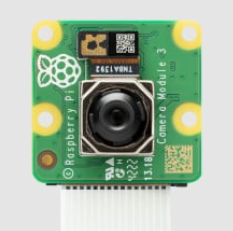
\includegraphics[width=0.5\linewidth]{figs/Raspberry Pi Camera Module V3.png}
    \caption{Figure of Raspberry Pi camera module 3. \citep{RP-DOC}}
    \label{fig:Raspberry Pi Camera Module 3}
\end{figure}

 The second most common failing criteria for camera modules was the focus depth of the camera modules. Since the distance from the camera module lens to the focus object is small, 5~mm to 100~mm, camera modules with large focus depth ranges are not practical for this project. This eliminated products from the hummingbird mobile camera module series, developed by Leopard  Imaging \citep{LI-P}, and the OV5647 spy camera module, developed by ArduCam. \citep{A-P}

Based on these two main selection criteria, two products have been selected to use for this project:

\begin{itemize}
    \item DF Robot 3-in-1 endoscope camera, produced by DF Robot.
    \item 1 MP 3.5~mm OV9734 HD endoscope medical camera module, produced by Vision Meta.
\end{itemize}

Table \ref{tab:DF vs VM} compares the two products mentioned above, while Figures \ref{fig:DF Robot} and \ref{fig:VM} illustrate the products.

\begin{table}[H]
    \centering
    \caption{DF Robot compared to Vision Meta.}
    \begin{tabular}{|c|c|c|}
    \hline
        \textbf{Feature} & \textbf{DF Robot} & \textbf{Vision Meta} \\
    \hline
        Diameter (mm) & 8 & 3.5  \\
    \hline
        Field of View (°) & 70 & 90 \\
    \hline
        Depth Focus (mm) & N/A & 5–100 \\
    \hline
        Resolution & 0.864 MP & 0.922 MP \\
    \hline
        Built-in LED & Yes & No \\
    \hline 
        Cost & R 457.70 & R 995.96 (\$60.00) \\
    \hline
        Shipping Cost & R0.00 & R 1 344.55 (\$81.00)\\
    \hline    
    \end{tabular}
    \label{tab:DF vs VM}
\end{table}

\begin{figure}[H]
    \centering
    
    
    \begin{subfigure}{0.45\textwidth}
        \centering
        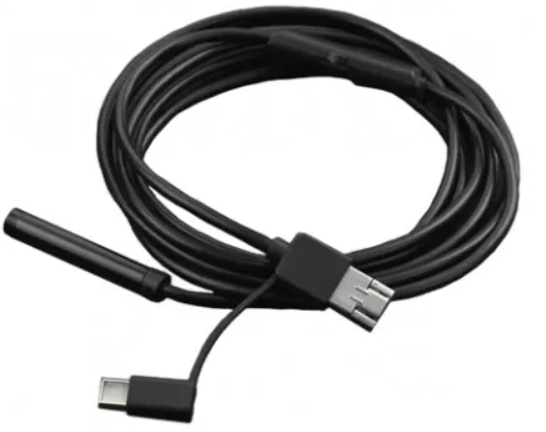
\includegraphics[width=\textwidth]{figs/DF Robot.png}
        \caption{DF Robot endoscope module. \citep{MR-P}}
        \label{fig:DF Robot}
    \end{subfigure}
    \hfill                          
    \begin{subfigure}{0.45\textwidth}
        \centering
        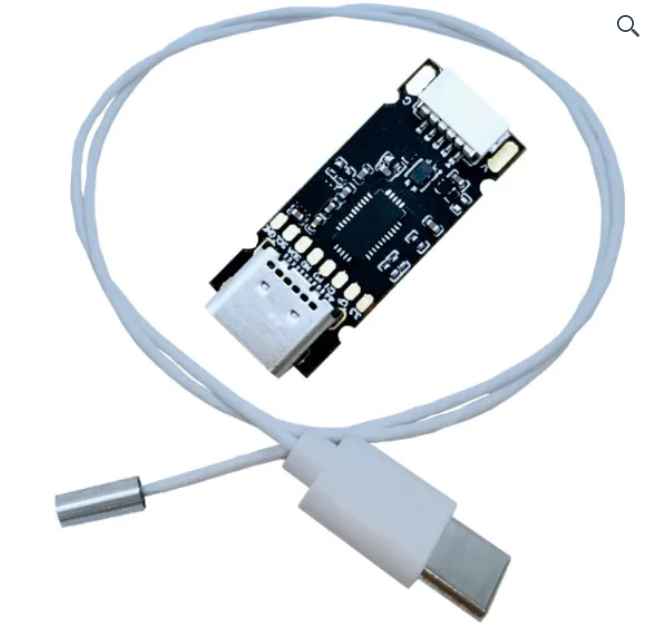
\includegraphics[width=\textwidth]{figs/Vision Meta.png}
        \caption{Vision Meta endoscope module. \citep{VM-P}}
        \label{fig:VM}
    \end{subfigure}

    \caption{Illustration of camera modules}
\end{figure}

These camera modules have USB compatibility and meet the physical specifications for this project and would, in theory, work. However, a feature that laparoscopes have is that the viewing angle is 30°. Due to the DF Robot endoscope’s large diameter and length, this feature makes it impractical for this project, unless the module is modified.

\subsection{Lighting Module}
\label{sec:Lighting Module}

Due to the laparoscopes being inserted into a patient’s body, there will be limited illumination within the patient, which will impact image quality. This can be easily resolved by installing illumination hardware on the laparoscope. These hardware components should be compact while producing enough illumination, which is measured in luminous intensity (cmd). Micro Robotics has two main products that can be used for this project. Both products are listed in Table \ref{tab:LED} and illustrated in Figure \ref{fig:LED}. \citep{MR-P}

\begin{table}[H]
    \centering
    \caption{List of illumination hardware. \citep{MR-P}}
    \begin{tabular}{|c|c|c|}
        \hline
            \textbf{Product} & \textbf{Luminous Intensity} & \textbf{Dimensions}\\
        \hline
            LED SMD 1206 & 200-850 cmd & 3.2 x 1.6 x 1.1 mm \\
        \hline
            LED SMD 0603 & 45-180 cmd & 1.6 x 0.8 x 0.55 mm \\
        \hline
        
    \end{tabular}
    \label{tab:LED}
\end{table}

\begin{figure} [H]
    \centering
    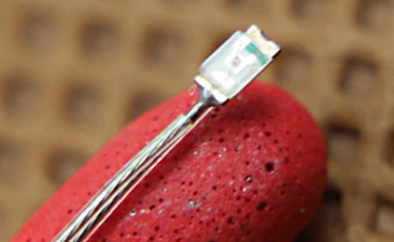
\includegraphics[height=3cm]{figs/LED.png}
    \caption{Figure of LED SMD 0603. \citep{MR-P}}
    \label{fig:LED}
\end{figure}

\subsection{Heat Transfer Components}
\label{sec:Heat Components}

The main purpose of the heat transfer components is to conduct heat from a direct or indirect heat source to a more suitable location, where the heat can either be dissipated naturally or forcefully to the environment. Therefore, there are two essential components that are required: A heat conduction medium and a heat sink.

The main purpose of a heat medium is to conduct heat from one location to another. Therefore, it requires a high conductivity value to be able to conduct the generated heat efficiently. The best commercial component design for this is a heat pipe. RS Components Ltd (RS) is a local supplier that has small-diameter heat pipes in stock, which would work for the laparoscope. Figure \ref{fig:Heat Pipe} depicts how a heat pipe looks.

\begin{figure}[H]
    
    \centering
    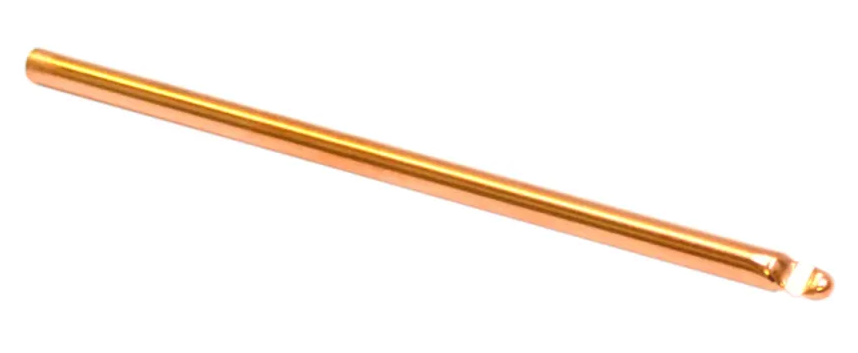
\includegraphics[height = 3 cm]{figs/Heat Pipe.png}
    \caption{Figure of a heat pipe. \citep{RS}}
    \label{fig:Heat Pipe}

\end{figure}

The heat sink's main purpose is to dissipate the heat conducted to it as effectively as possible. It accomplishes this through its design, where the surface area of the component is maximized. RS Components holds various heat sink models also in stock, which will satisfy the need for the laparoscope. 

A third component can be added to the design if it is required. If natural convection is not effective enough to dissipate heat from the heat sinks, then forced convection should be considered. This is accomplished through the means of a fan that blows cold air onto the heat sinks, while an additional fan extracts the hot air away from the heat sinks. RS Components also holds a large variety of fans that can suffice for this project. \citep{RS}


\section{Software Considerations}
\label{sec:Software Considerations}

 The most important software consideration of this project is that of the camera module interface. Since both camera modules that are going to be used in this project use a USB interface, the recommended software to operate the camera modules is AMCap.  \citep{MR-P} However, Open CV can also be utilized to control USB camera modules.


The software language is an important aspect that needs to be considered. However, this is dependent on the SBC used. If a Raspberry Pi is used, then Python is the recommended language to use. \citep{RP-DOC} However, if an Arduino is used, then the recommended language to use is either C or C++. \citep{A-DOC} Visual Studio Code (VS Code) can be used to perform all programming for this project.

% Documentation of this project will be performed using LaTeX. VS Code will be used to run this application, through the LaTeX Workshop extension.\citep{VS-LW}

\section{Visual Inspection Considerations}
\label{sec:Visual Inspection Considerations}

This project requires a camera to be a functional laparoscope. However, there are various factors to be considered to take high‑quality images. This section of the literature review aims to explain each of these factors.  

An important concept to understand is how a digital image is captured. A camera sensor consists of a matrix of millions of light cavities. When a picture is being taken, these cavities, called "photosites", are exposed to the photons of the object or scene. The photons are then collected by the photosites and stored as an electrical charge. Consequently, when the image is taken, these charges are quantified and then processed to form the image. \citep{CC-DCS}

One aspect that needs to be mastered to capture quality images is the exposure triangle. This triangle consists of three pillars that dictate the quality of an image. The first pillar, called aperture, determines the size of the area opened in the lens through which light can filter through to the sensor. The larger the aperture value, measured in f‑stop values, the smaller the hole size through which light filters through the lens. These pillars relate to the depth of field of the images. The smaller aperture correlates to shallower depth of field images. \citep{CC-CE}

Shutter speed is the second pillar of the exposure triangle. When a digital image is being taken, the lens opens up to expose the photosites to the light. Consequently, shutter speed refers to the total duration of the lens being open. If the shutter speed increases, then the sensors are exposed to a reduced duration of light from the images. Therefore, as the shutter speed increases, the images will gain more quality, with more definitive objects that are more "frozen" in the image. \citep{CC-CE}

The third pillar is ISO. This determines how sensitive the sensor is to the exposed light. As the ISO value increases, the sensitivity value will become higher. Therefore, the image will have increased levels of noise captured if the ISO value is increased.  \citep{CC-CE}

Focal length is a critical feature that has to be considered for this project. Focal length is the distance between the camera sensor and the focal lens. As this value increases, the field of view value will decrease. Field of view, measured in degrees, is essentially how much of a scene can be seen. If this value increases, then a wider image can be taken \citep{DM-FOW}






